\chapter{Introduction}


\section{Motivation}

Modern computer vision and graphics applications -- from AR/VR systems to robotics and real-time rendering -- depend critically on 3D scene representations that are both compact and geometrically accurate. In AR/VR, for instance, convincing user experiences require precise geometry: objects must stay anchored in place, occlusions need to look correct, and the overall spatial structure must remain stable under user movement. At the same time, these systems operate under strict real-time and memory constraints, so representations cannot be arbitrarily large or slow to process. Current 3D Gaussian Splatting approaches often require 500+ MB per scene, making them impractical for deployment on mobile devices or real-time streaming applications. Similar demands arise in robotics, where reliable 3D understanding directly impacts localization, path planning, and safe interaction with the environment -- errors in geometry can have tangible consequences. Likewise, in graphics pipelines tasked with rendering complex scenes, the representation must scale efficiently without sacrificing visual quality.

Recent neural rendering methods have made impressive strides in synthesizing novel views from sparse image sets. Techniques such as Neural Radiance Fields (NeRFs)~\cite{mildenhall2020nerf} and, more recently, 3D Gaussian Splatting (3DGS)~\cite{kerbl20233dgs}, can produce highly photorealistic images by learning scene representations directly from photographs. 3DGS, in particular, stands out for its real-time rendering performance and memory efficiency, making it attractive for interactive and large-scale applications. However, these methods are primarily optimized for appearance fidelity rather than explicit geometric correctness.

A key challenge is that depth and surface structure emerge implicitly in these models rather than being explicitly enforced. Without strong geometric supervision, reconstructed scenes often suffer from depth inconsistencies across viewpoints, incorrect scale, and poorly defined surfaces, especially in challenging regions such as textureless walls or repetitive patterns. Individual primitives are optimized largely independently, which can result in fragmented or noisy surface reconstructions that appear acceptable in rendered images but degrade when evaluated geometrically. As a result, while neural rendering techniques excel at visual synthesis, the underlying 3D structure is frequently unreliable for applications that require accurate surface reconstruction or metrically consistent representations.

Figure~\ref{fig:normal_comparison_intro} makes the geometric quality problem concrete. Surface normal maps encode per-pixel surface orientation and expose geometric inconsistencies that are invisible in standard RGB renders. The red-boxed region is the same across all methods and reveals a clear progression: standard 3DGS produces incoherent, structureless normals in areas that should be flat walls — a sign that the underlying geometry is noisy and fragmented. Many recent methods attempt to address this through geometry-aware initialization (GeoGaussian), planar constraints (PlanarGS), and other structural regularization strategies, each making measurable progress. Our goal in this thesis is not to outperform state-of-the-art methods in rendering quality, but to demonstrate that comparable geometric fidelity can be achieved at a fraction of the storage cost — 222~MB versus 740~MB for vanilla 3DGS — through principled integration of geometric priors and edge-aware adaptive densification.

\begin{figure}[t]
    \centering
    \setlength{\tabcolsep}{2pt}
    \renewcommand{\arraystretch}{0.5}
    \begin{tabular}{cccc}
        \small View 1 & \small View 3 & \small View 4 & \small View 5 \\[2pt]
        % Ground Truth row
        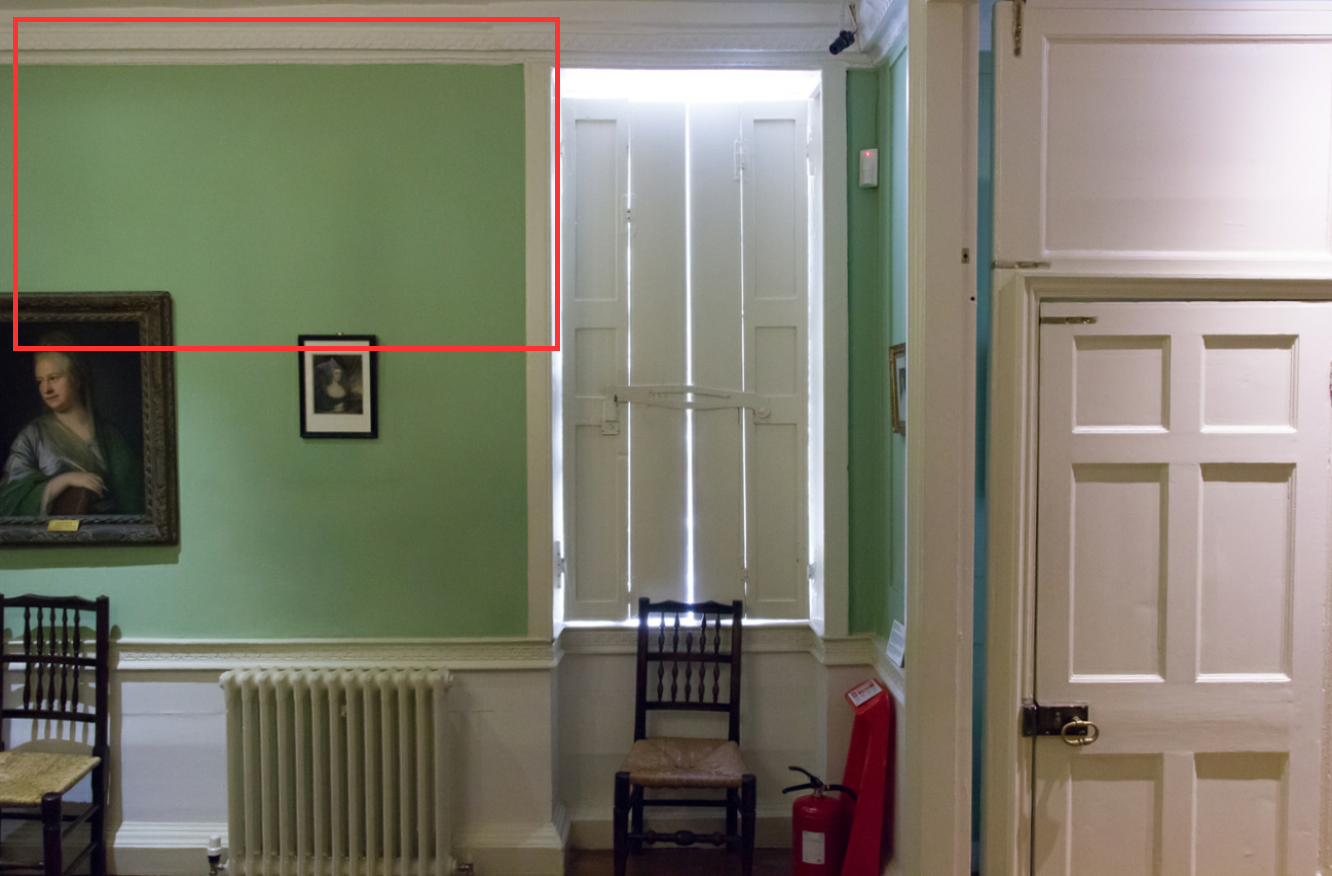
\includegraphics[width=0.235\textwidth]{comparison_figures/drjohnson_gt_view01_rect.png} &
        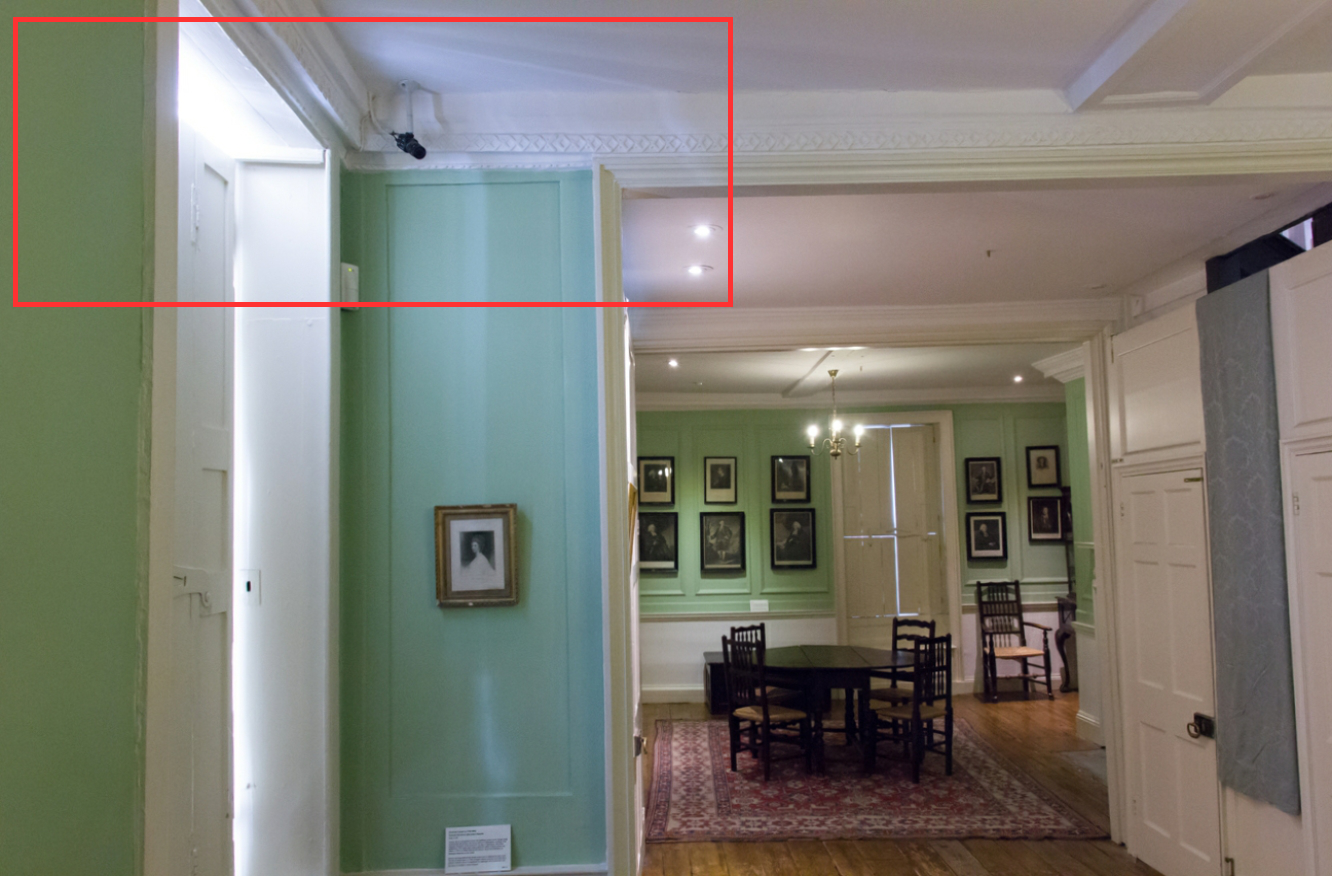
\includegraphics[width=0.235\textwidth]{comparison_figures/drjohnson_gt_view03_rect.png} &
        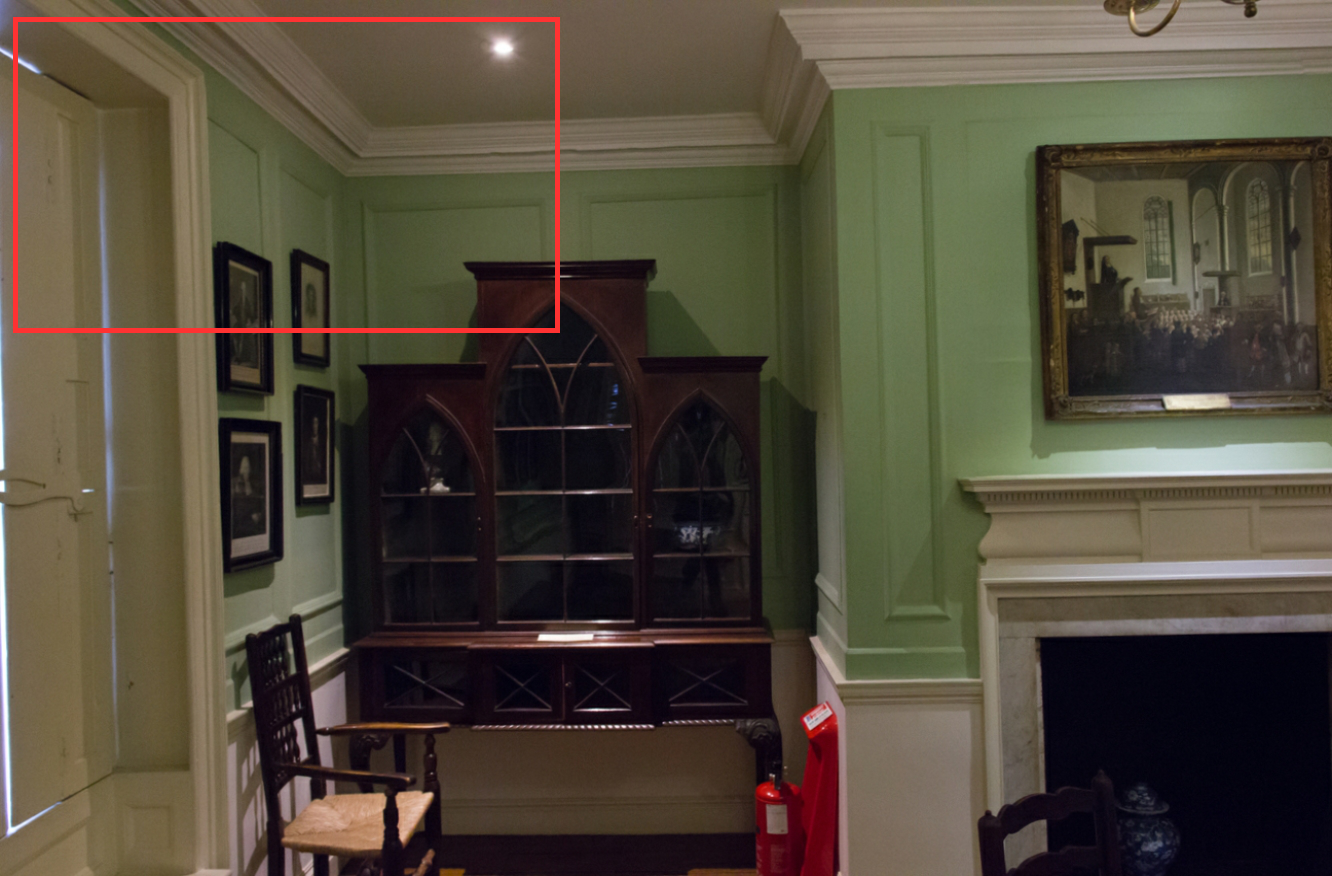
\includegraphics[width=0.235\textwidth]{comparison_figures/drjohnson_gt_view04_rect.png} &
        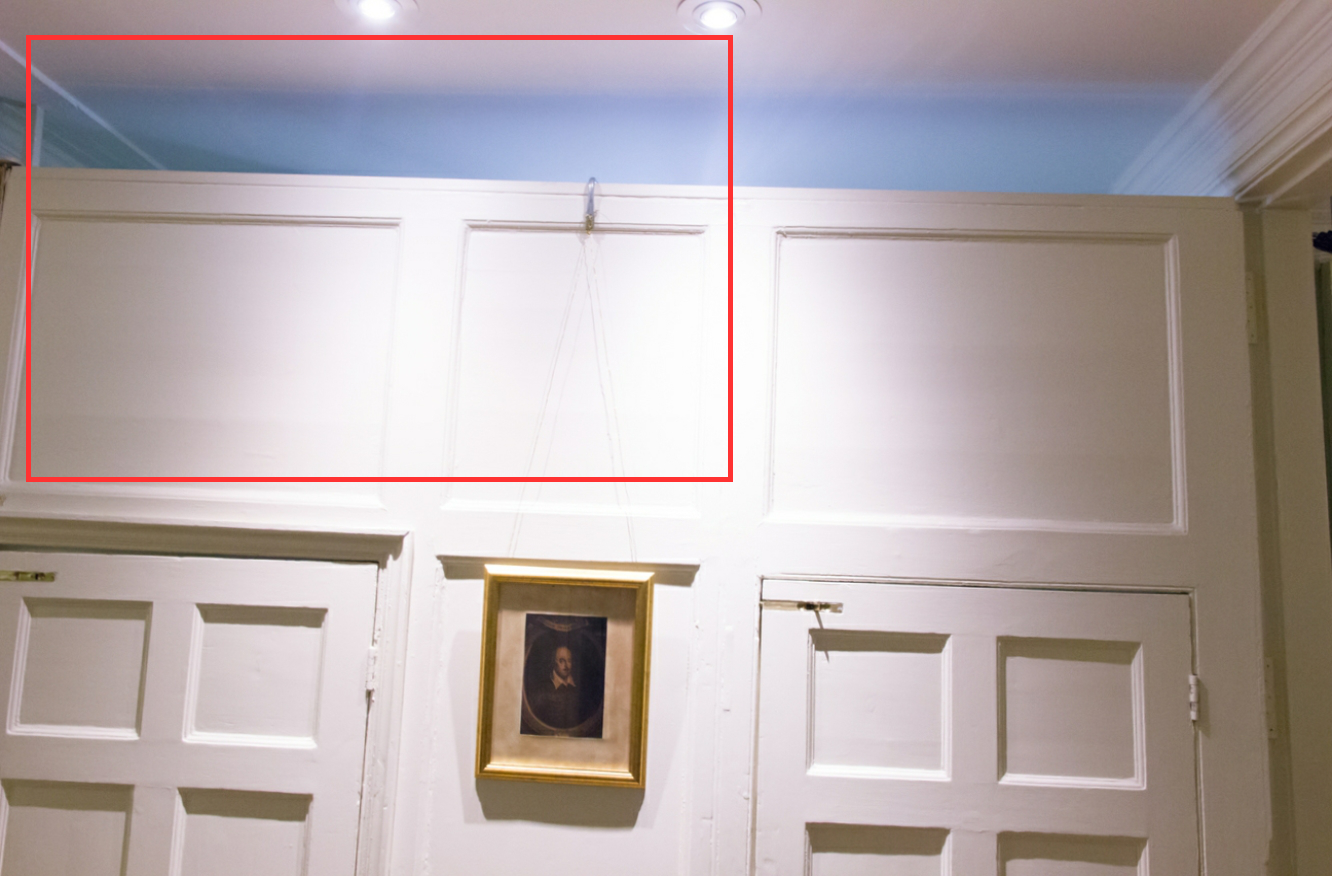
\includegraphics[width=0.235\textwidth]{comparison_figures/drjohnson_gt_view05_rect.png} \\
        \multicolumn{4}{c}{\small\textbf{(a) Ground Truth}} \\[4pt]
        % 3DGS normals
        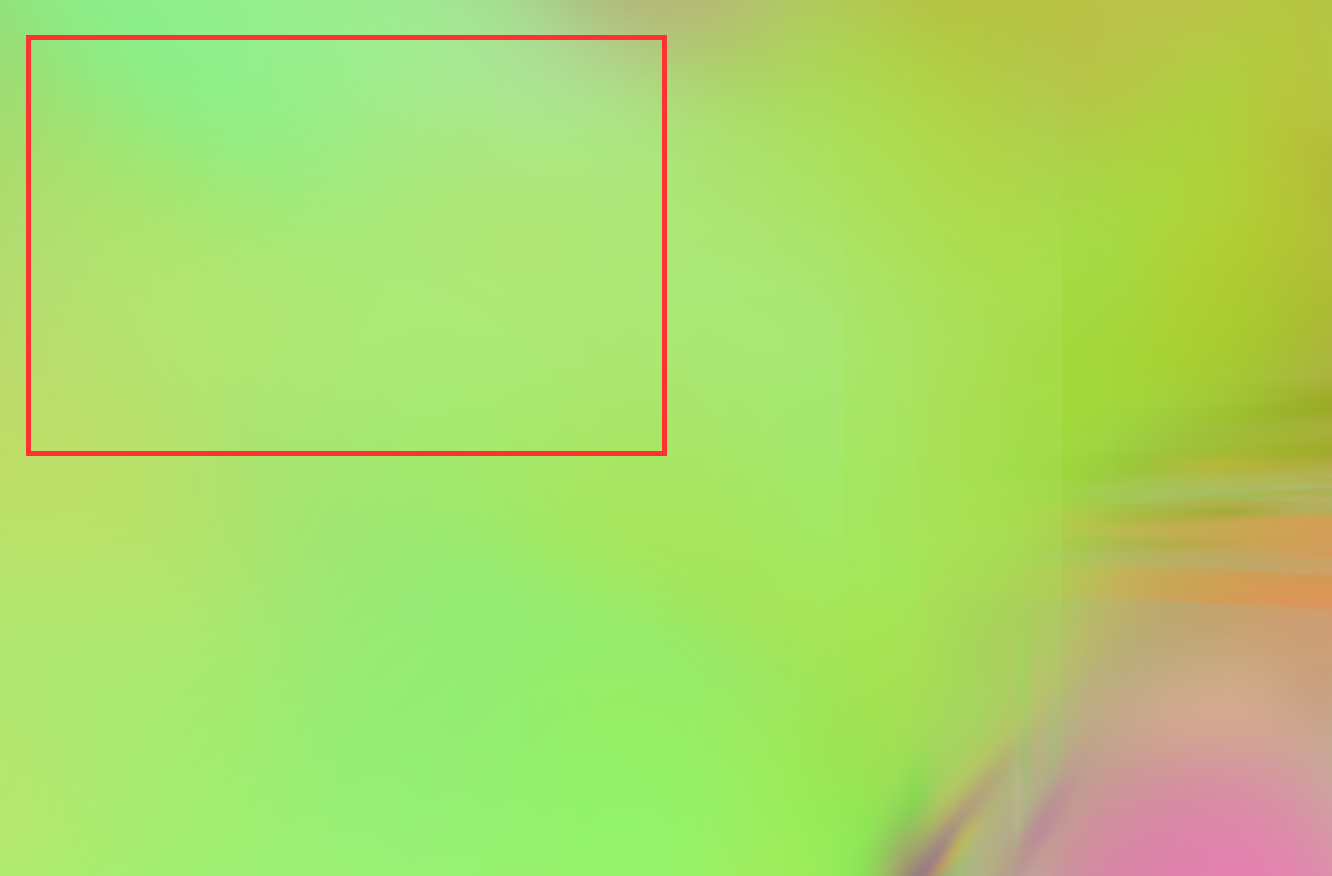
\includegraphics[width=0.235\textwidth]{comparison_figures/normal_view01_3DGS_rect.png} &
        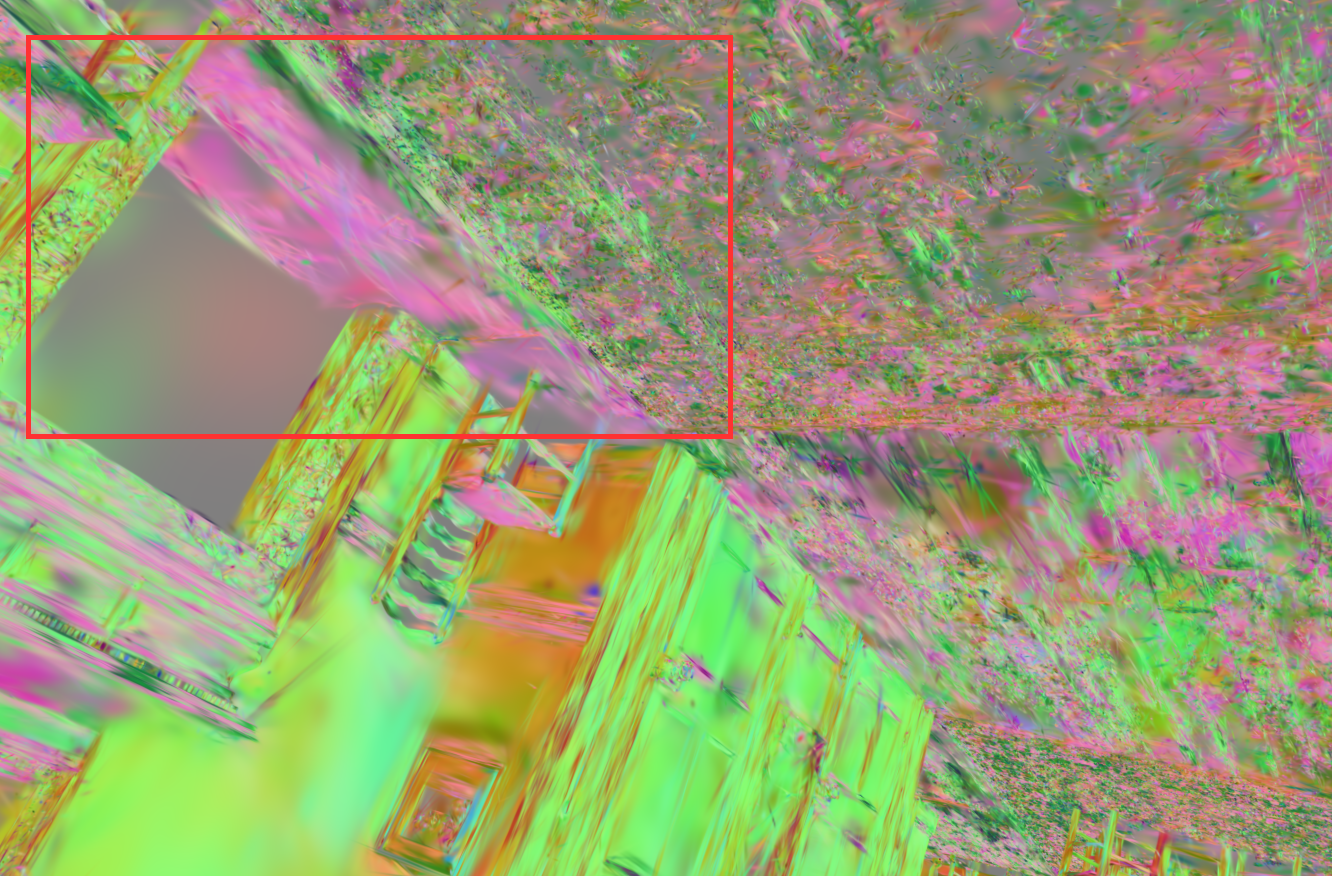
\includegraphics[width=0.235\textwidth]{comparison_figures/normal_view03_3DGS_rect.png} &
        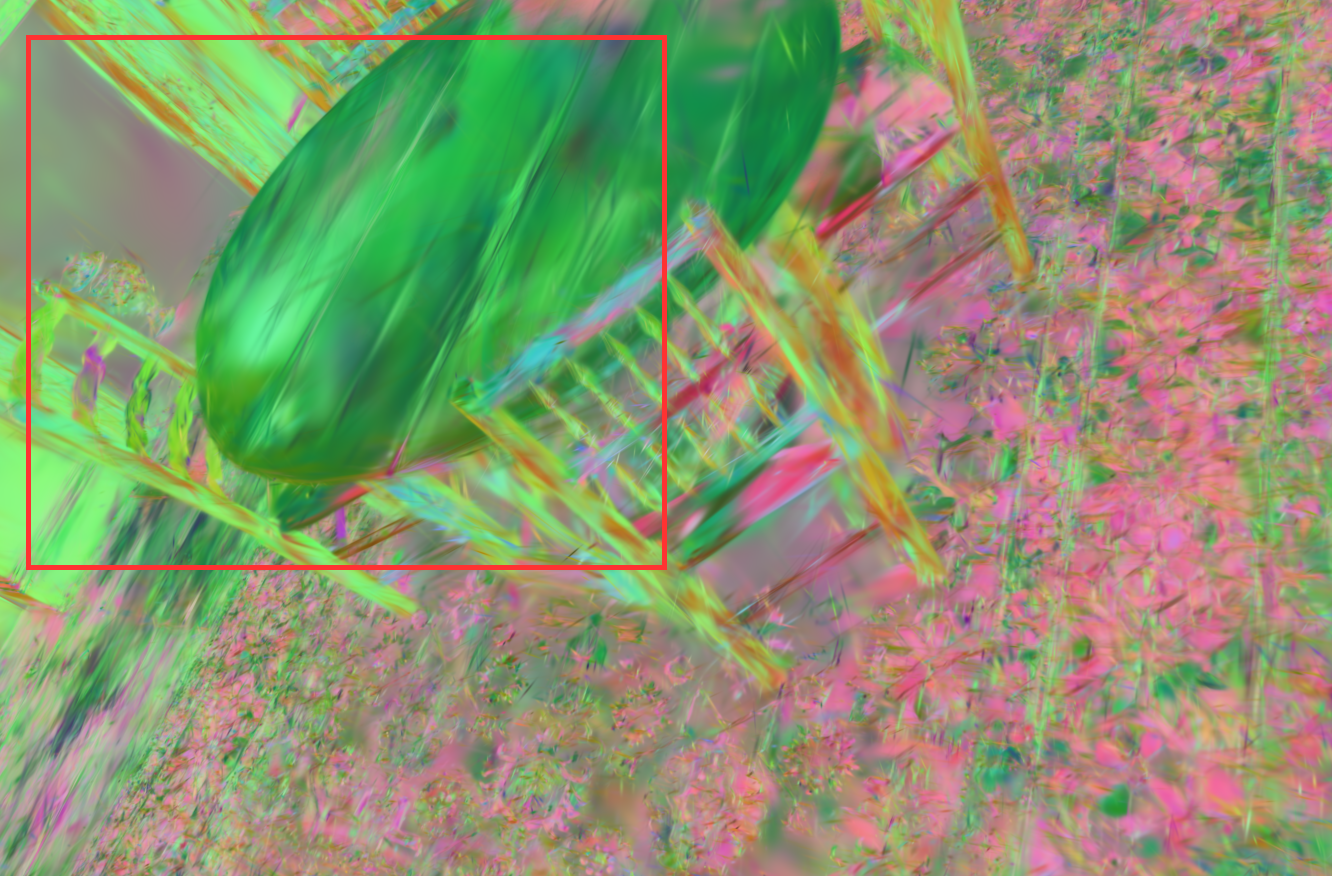
\includegraphics[width=0.235\textwidth]{comparison_figures/normal_view04_3DGS_rect.png} &
        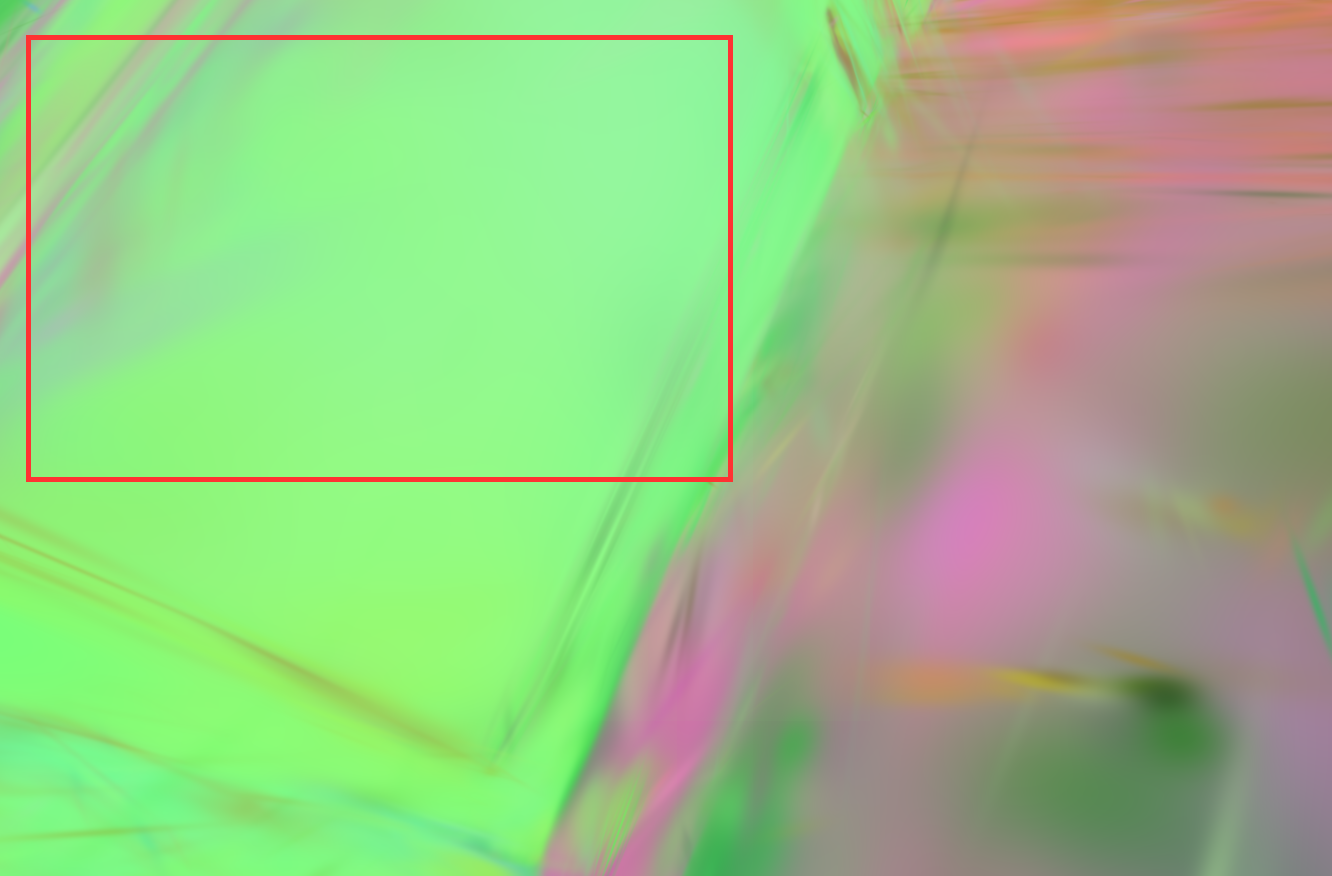
\includegraphics[width=0.235\textwidth]{comparison_figures/normal_view05_3DGS_rect.png} \\
        \multicolumn{4}{c}{\small\textbf{(b) 3D Gaussian Splatting} — 740 MB} \\[4pt]
        % GeoGaussian normals
        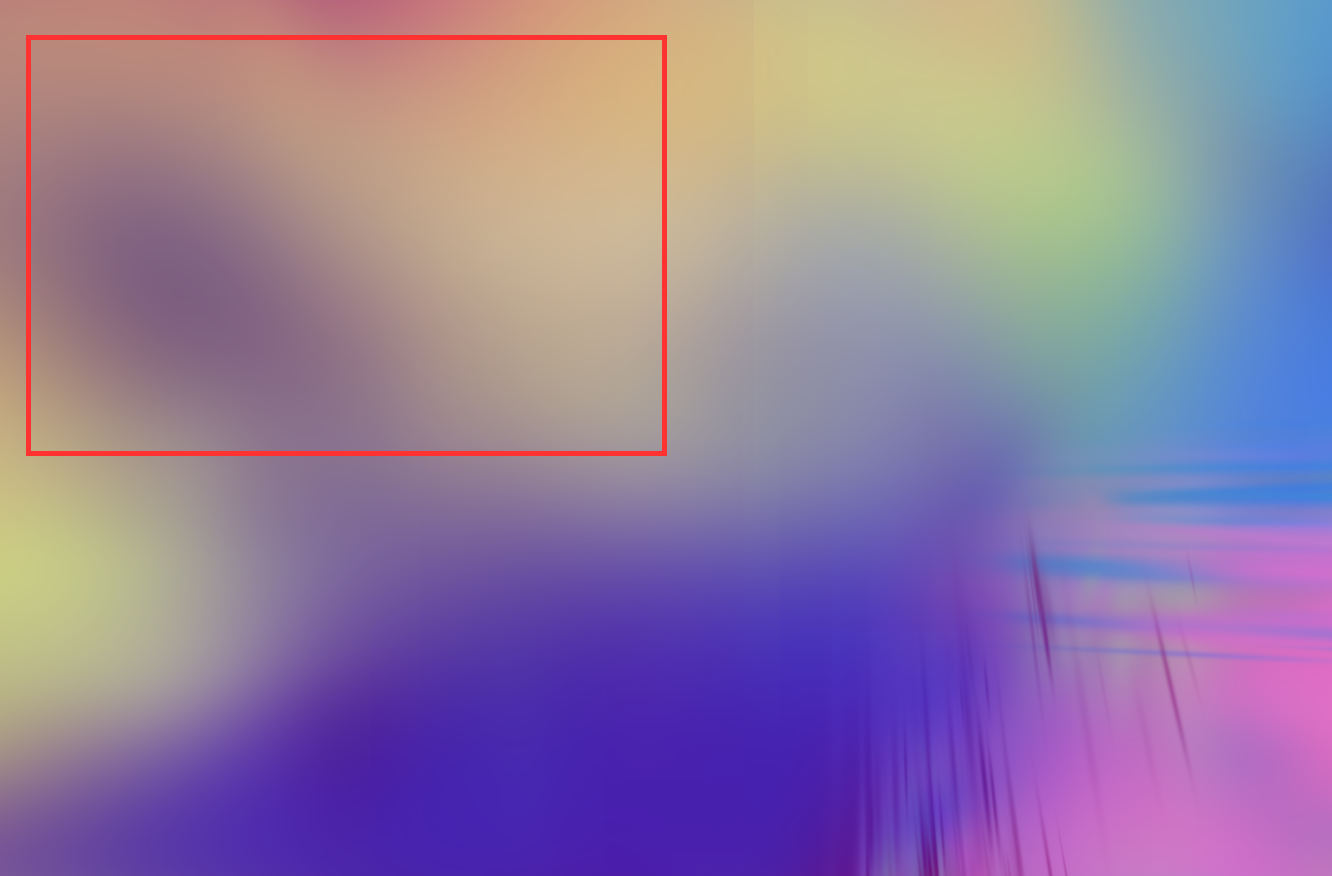
\includegraphics[width=0.235\textwidth]{comparison_figures/normal_view01_GeoGaussian_rect.png} &
        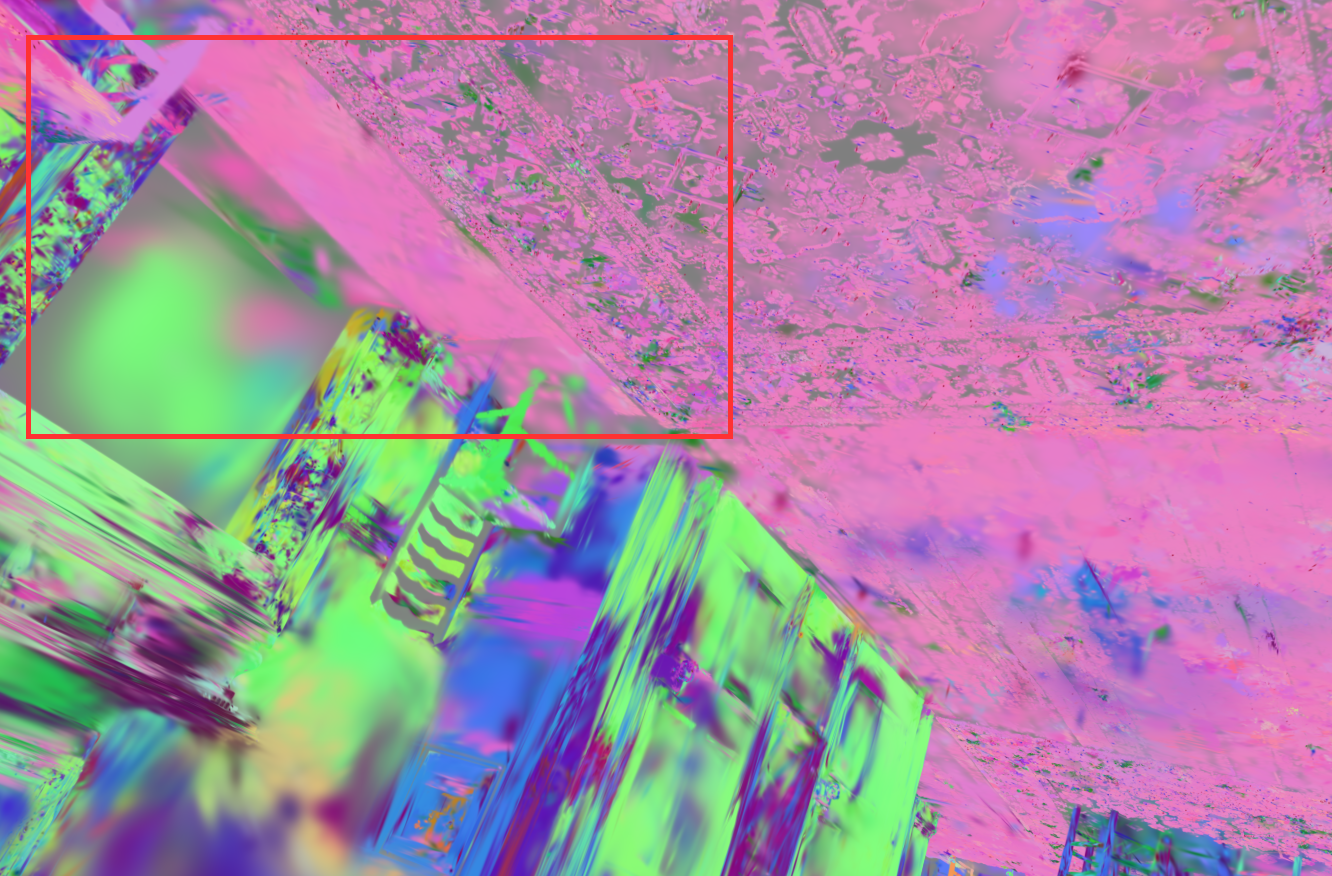
\includegraphics[width=0.235\textwidth]{comparison_figures/normal_view03_GeoGaussian_rect.png} &
        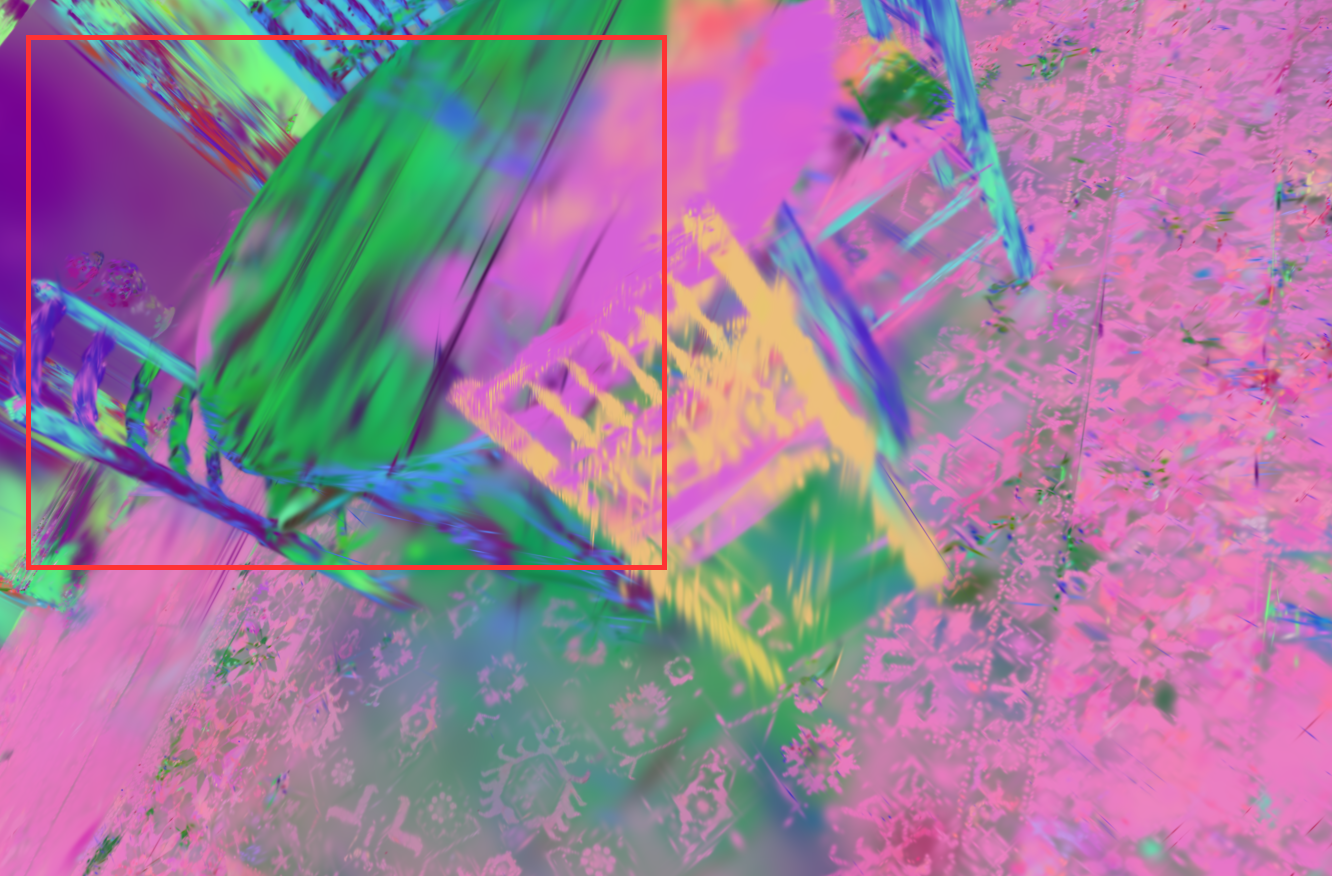
\includegraphics[width=0.235\textwidth]{comparison_figures/normal_view04_GeoGaussian_rect.png} &
        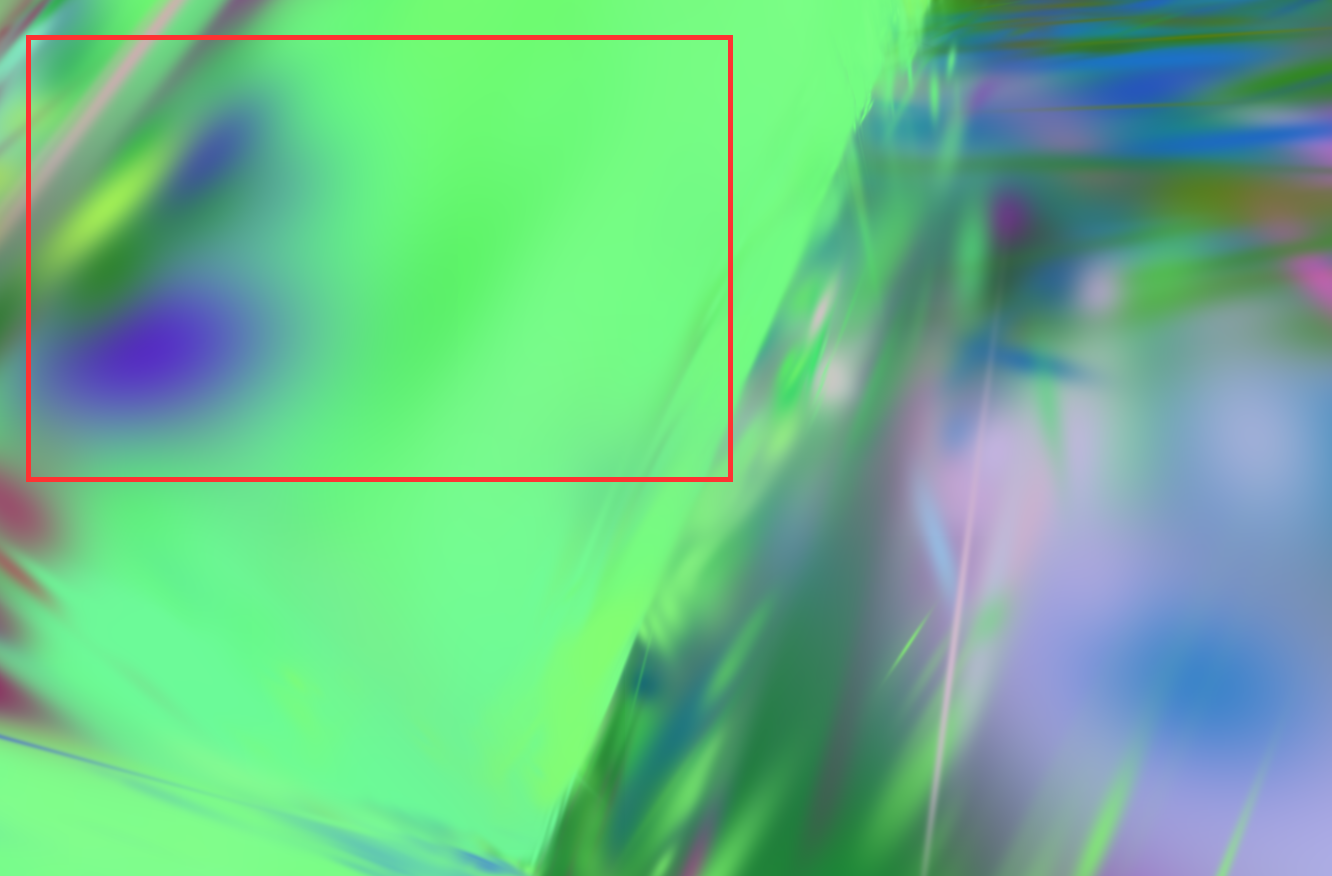
\includegraphics[width=0.235\textwidth]{comparison_figures/normal_view05_GeoGaussian_rect.png} \\
        \multicolumn{4}{c}{\small\textbf{(c) GeoGaussian} — 281 MB} \\[4pt]
        % PlanarGS normals
        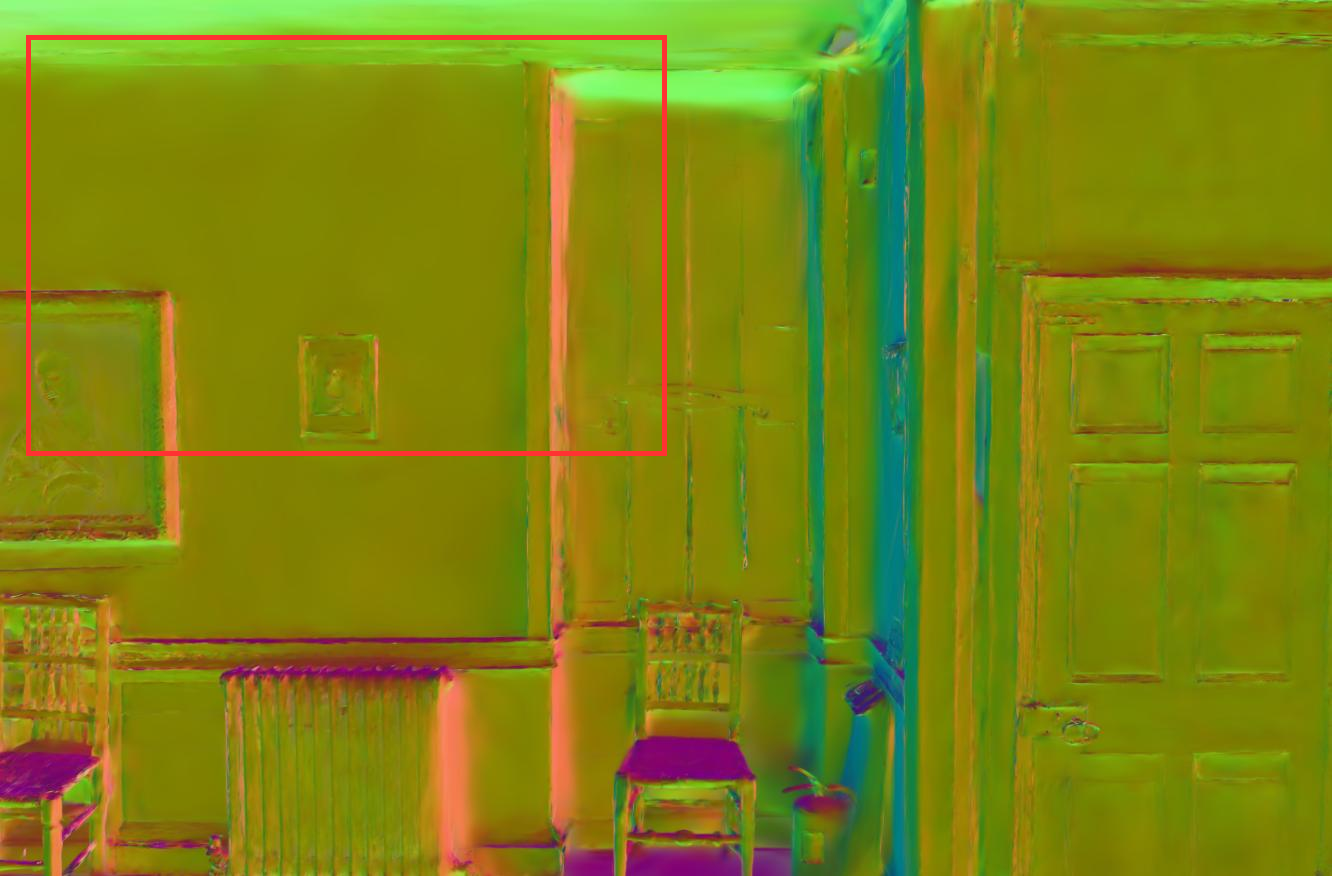
\includegraphics[width=0.235\textwidth]{comparison_figures/normal_view01_PlanarGS_rect.png} &
        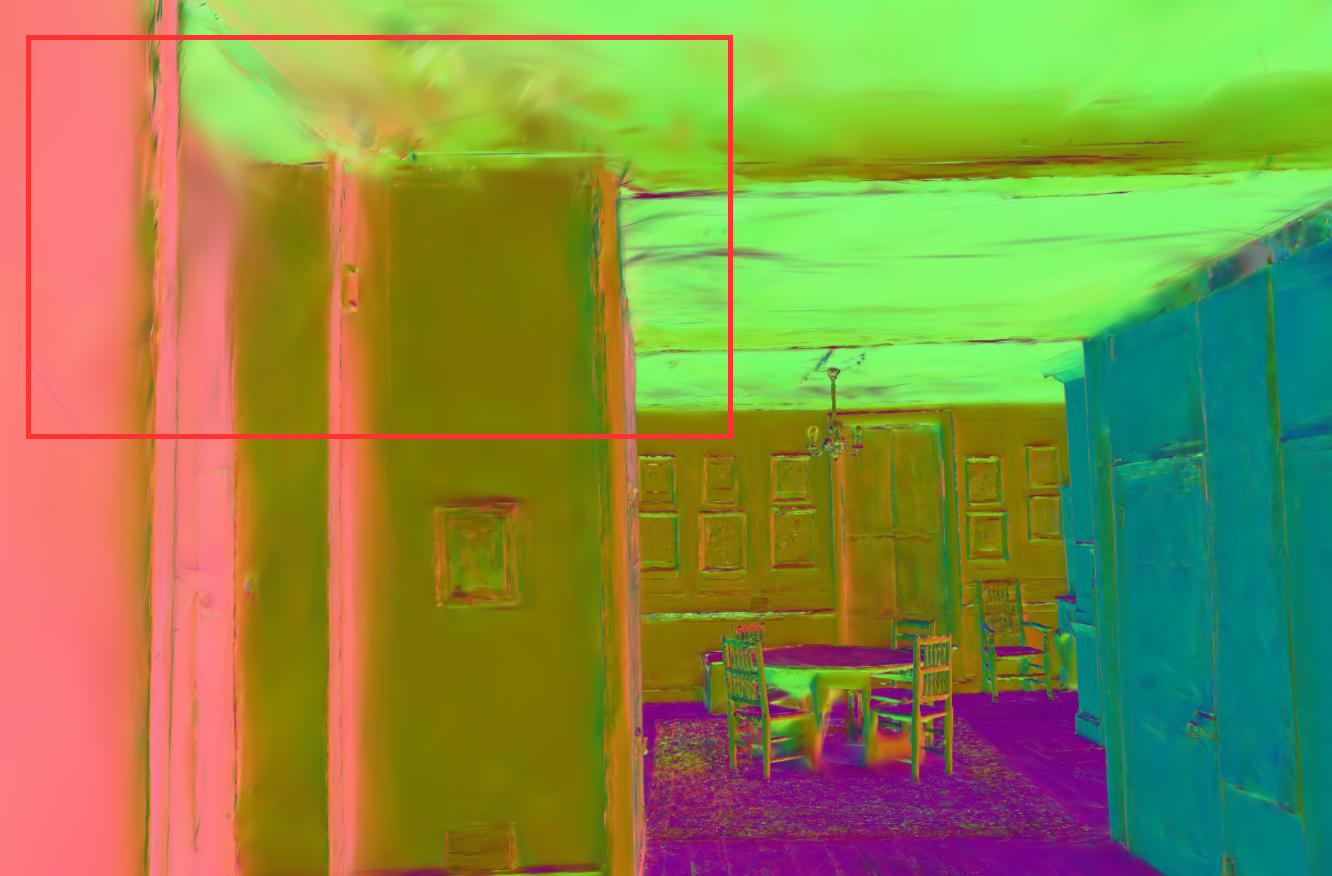
\includegraphics[width=0.235\textwidth]{comparison_figures/normal_view03_PlanarGS_rect.png} &
        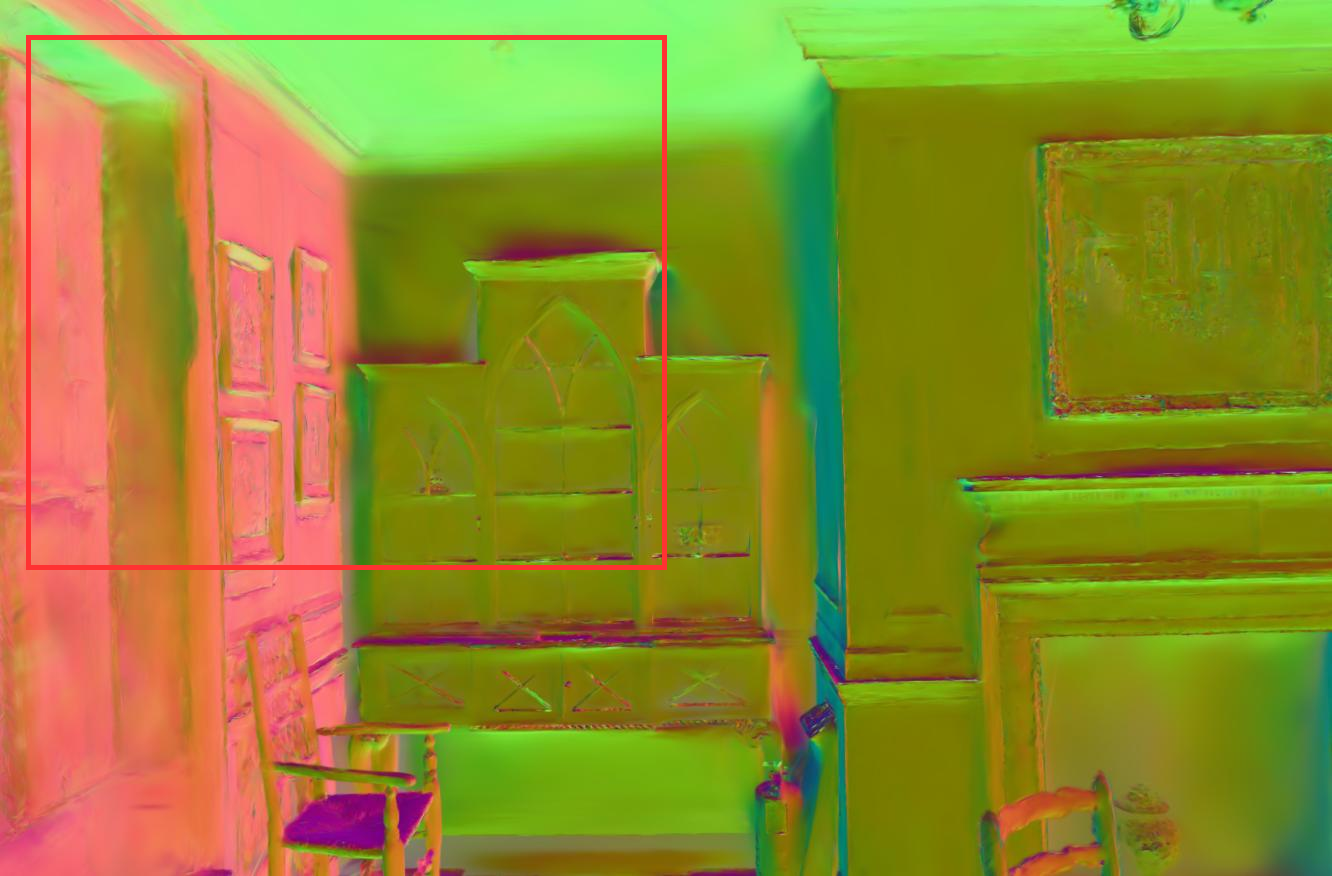
\includegraphics[width=0.235\textwidth]{comparison_figures/normal_view04_PlanarGS_rect.png} &
        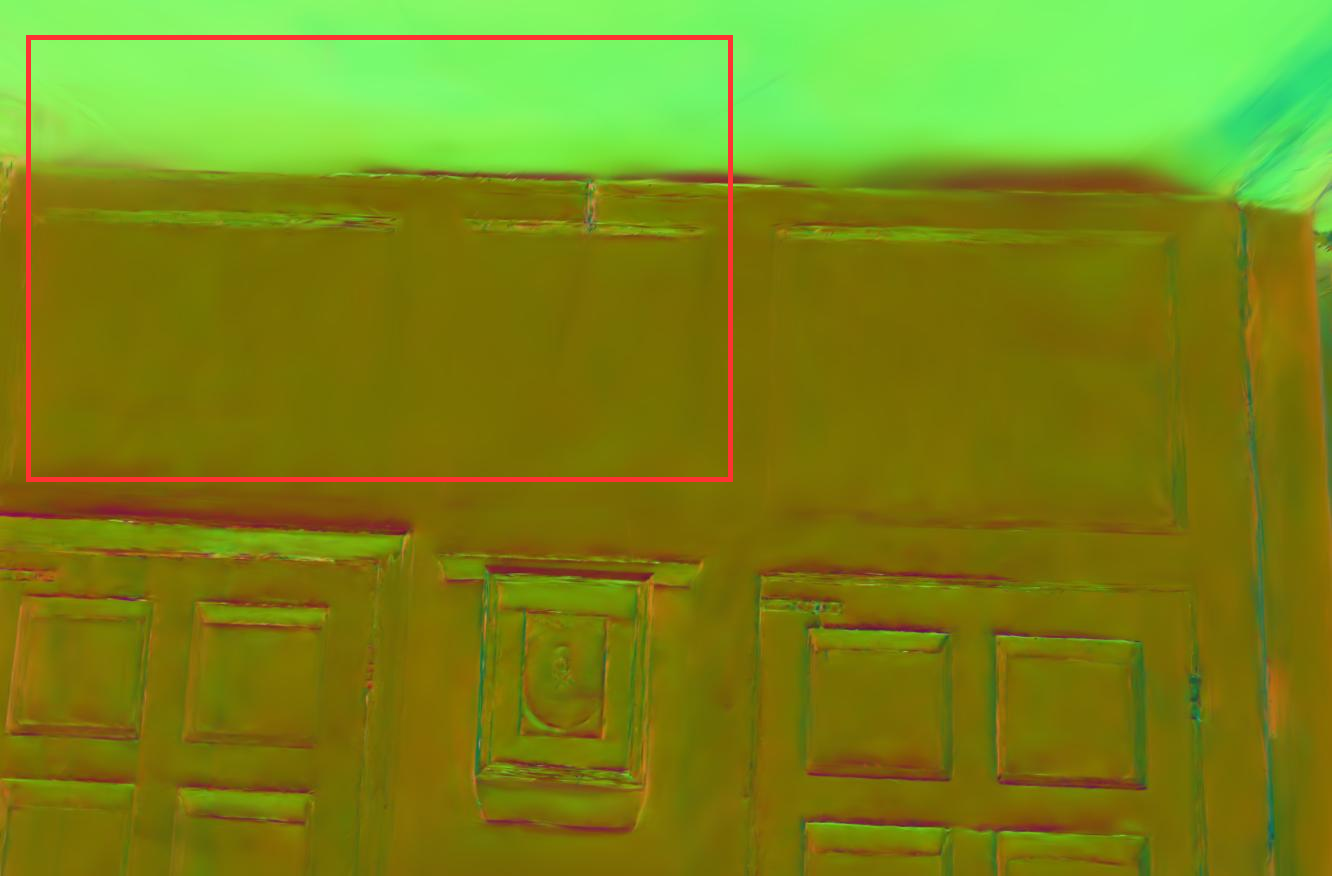
\includegraphics[width=0.235\textwidth]{comparison_figures/normal_view05_PlanarGS_rect.png} \\
        \multicolumn{4}{c}{\small\textbf{(d) PlanarGS} — 410 MB} \\[4pt]
        % Ours normals
        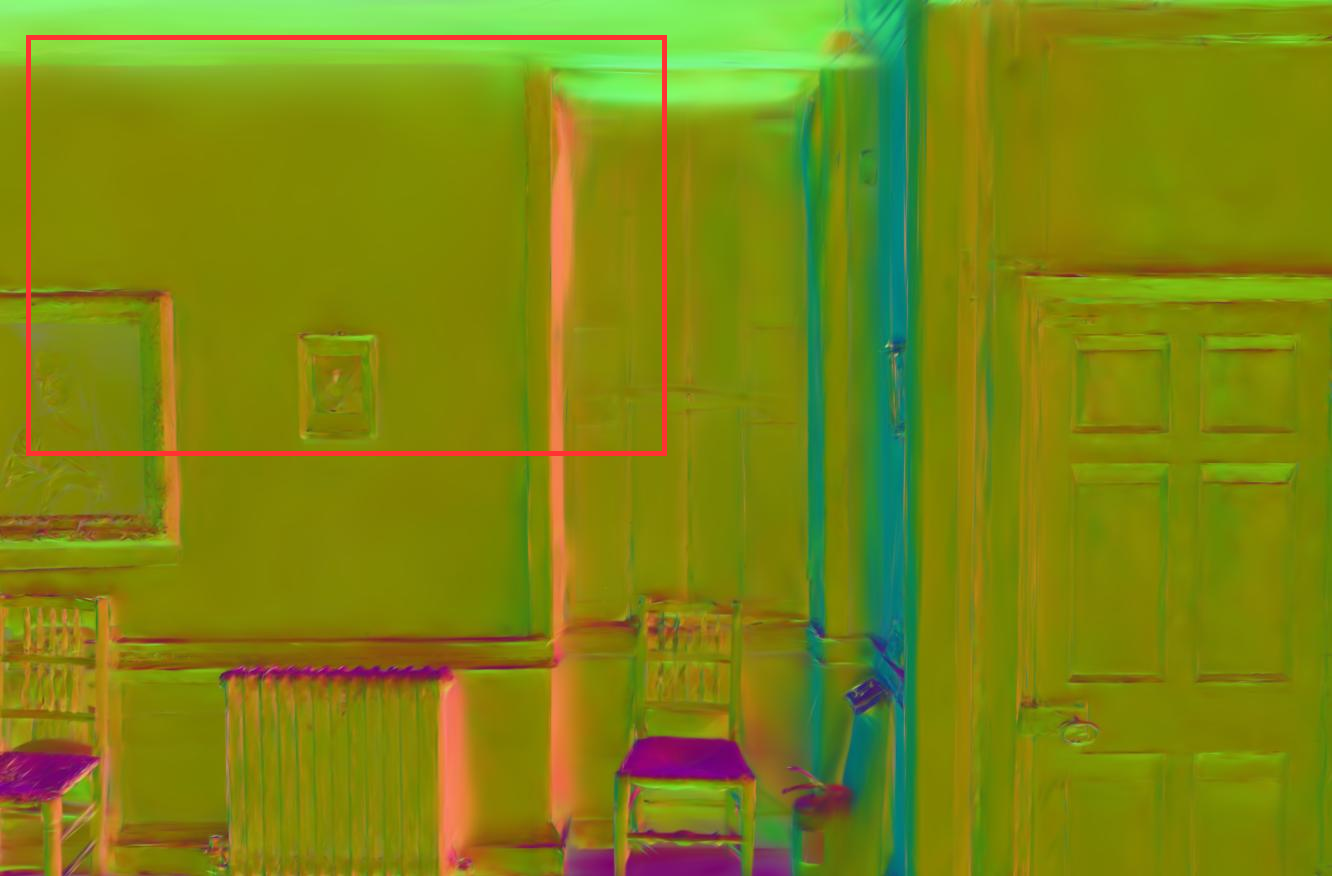
\includegraphics[width=0.235\textwidth]{comparison_figures/normal_view01_Ours_rect.png} &
        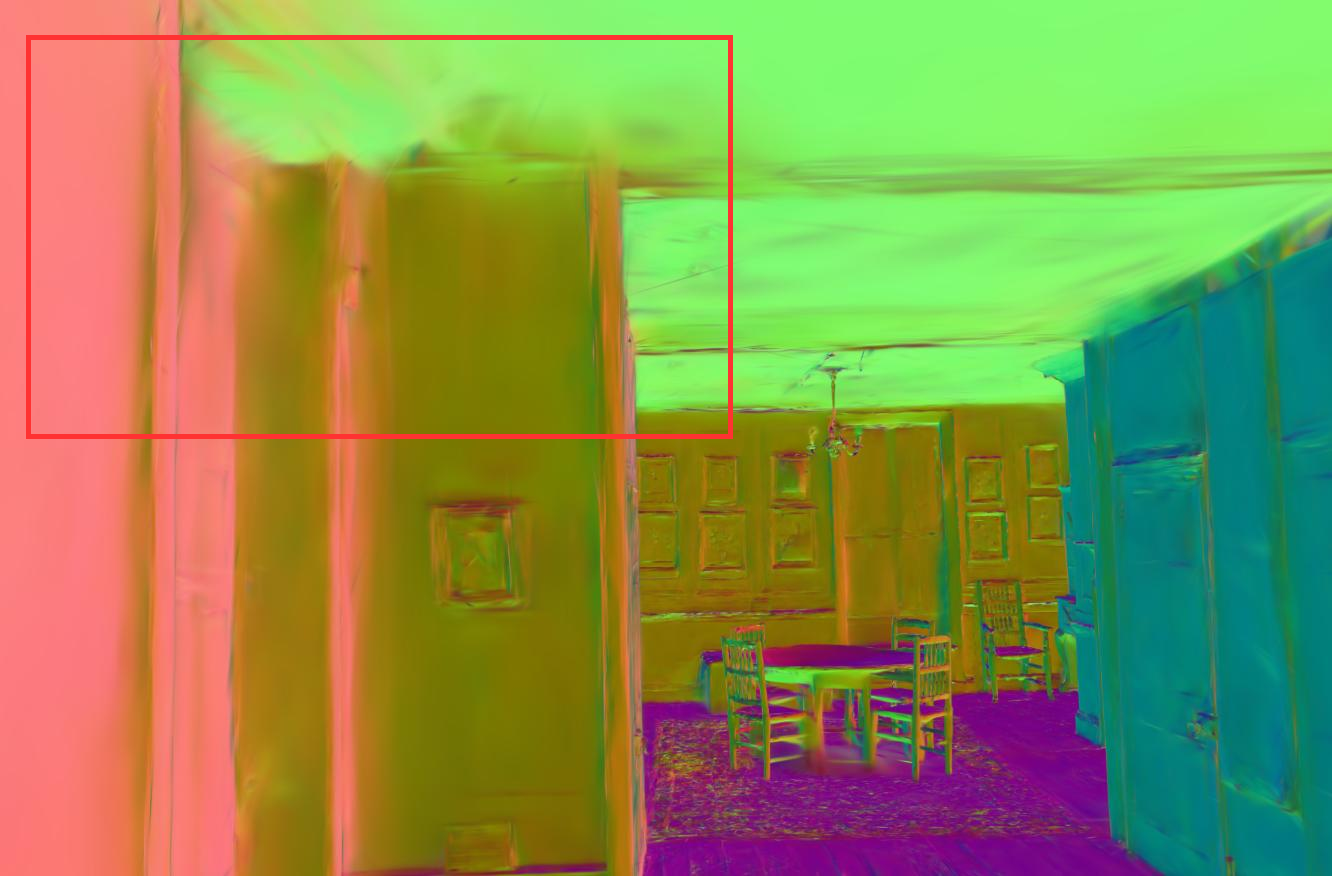
\includegraphics[width=0.235\textwidth]{comparison_figures/normal_view03_Ours_rect.png} &
        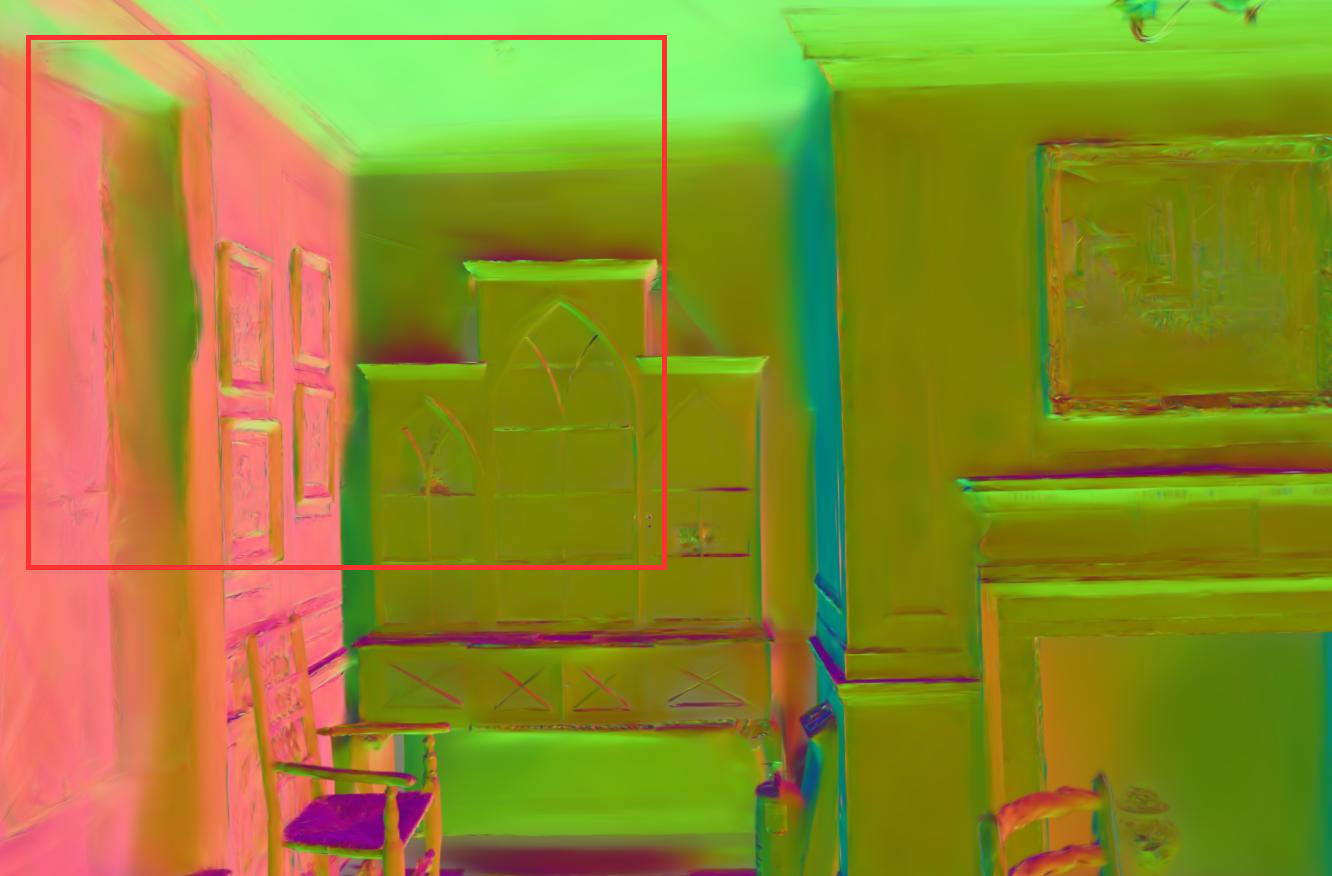
\includegraphics[width=0.235\textwidth]{comparison_figures/normal_view04_Ours_rect.png} &
        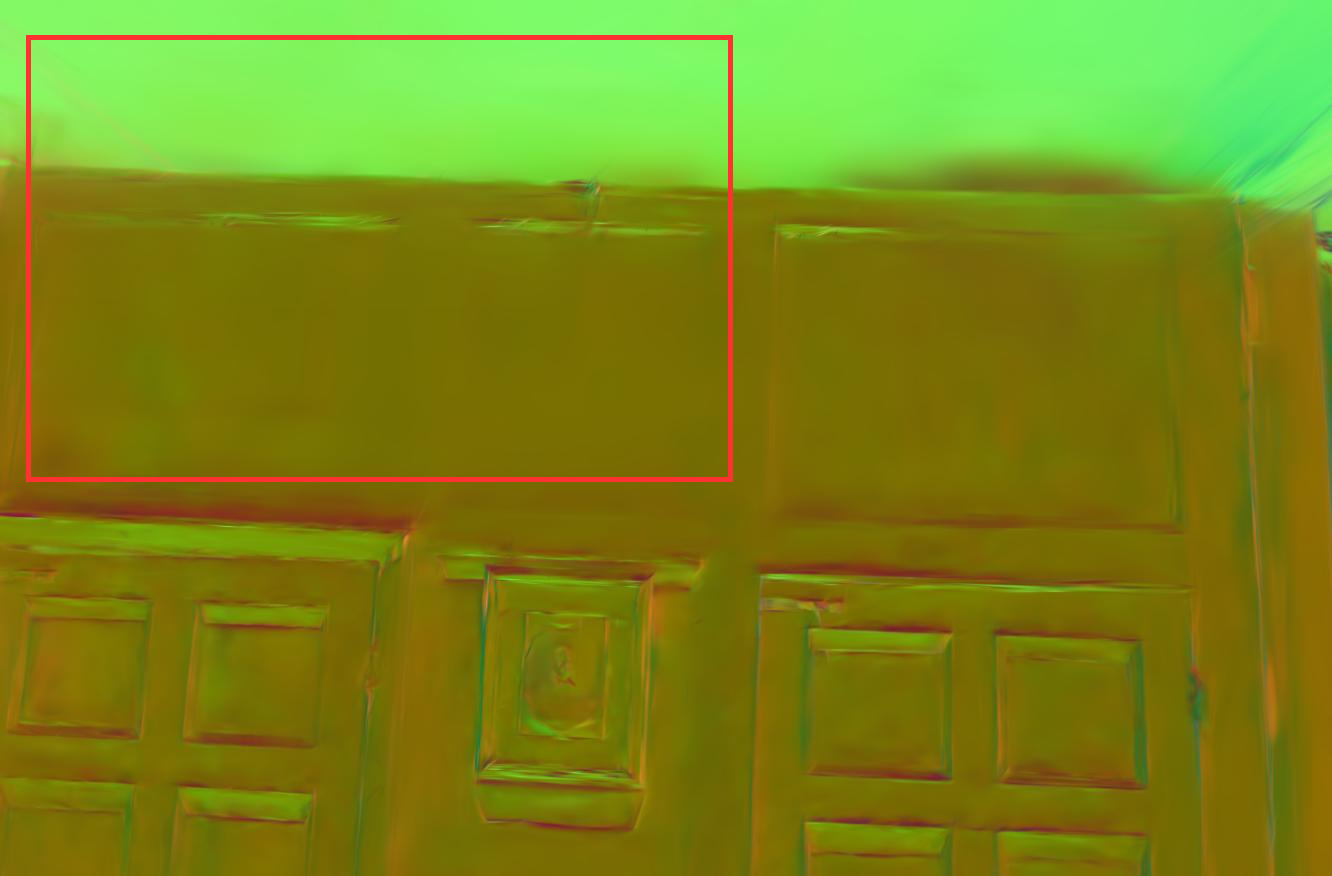
\includegraphics[width=0.235\textwidth]{comparison_figures/normal_view05_Ours_rect.png} \\
        \multicolumn{4}{c}{\small\textbf{(e) Ours (PlanarGS + edge-aware)} — 222 MB} \\
    \end{tabular}
    \caption{Surface normal maps rendered from four DrJohnson viewpoints. Row~(a) shows ground truth RGB images for reference. Rows~(b)--(e) show rendered normals, which directly encode per-pixel surface orientation and reveal geometric quality differences that are invisible in RGB renders. The red rectangle marks the same region across all methods. Standard 3DGS (b) produces incoherent normals with no discernible surface structure in the highlighted region. GeoGaussian (c) shows improvement from geometry-aware initialization but remains noisy. PlanarGS (d) achieves visibly cleaner planar normals. Our method (e) produces the most coherent surfaces, matching PlanarGS quality while storing the scene in only 222~MB — 70\% less than 3DGS.}
    \label{fig:normal_comparison_intro}
\end{figure}

The central question this thesis addresses is: \textit{which geometric priors, individually and in combination, provide the most effective path toward compact yet geometrically faithful 3D Gaussian Splatting representations for structured indoor scenes?}

\section{Contributions}

The contributions of this thesis are summarized as follows:

\begin{itemize}
    \item \textbf{Unified geometry-aware framework:} We propose a unified geometry-aware 3D Gaussian Splatting framework that integrates five complementary geometric modalities: normal priors, depth priors, planar co-planarity constraints, mesh-based regularization through TSDF fusion, and edge-aware adaptive densification. The framework is fully modular, allowing each component to be independently enabled or disabled through command-line flags, facilitating systematic ablation analysis. This design builds upon and extends ideas from GeoGaussian~\cite{geogaussian}, DN-Splatter~\cite{dn_splatter}, PlanarGS~\cite{planargs}, SuGaR~\cite{sugar}, and MILO~\cite{milo2024}, unifying them into a single cohesive pipeline.

    \item \textbf{Comprehensive ablation study across 32 configurations:} We conduct the first comprehensive ablation study that systematically evaluates all $2^5 = 32$ possible combinations of geometric priors (normals, depth, planarity, mesh constraints, and edge-aware control). This systematic exploration quantifies the individual and combined impact of each modality on reconstruction quality, representation compactness, and training efficiency. The study reveals important insights about redundancy, complementarity, and optimal combinations of geometric regularization strategies.

    \item \textbf{Edge-aware adaptive densification:} We introduce a novel edge-aware adaptive densification mechanism that concentrates smaller Gaussians near structural boundaries while using larger, more efficient primitives in planar interiors. This spatially varying strategy improves both geometric fidelity at edges and representation compactness in homogeneous regions, reducing the total primitive count by 30--32\% while maintaining or improving visual quality.

    \item \textbf{Experimental evaluation and practical insights:} We present extensive experimental evaluation on three indoor scenes from the Deep Blending dataset (DrJohnson, Library, and Playroom), using standard metrics (PSNR, SSIM, LPIPS) alongside efficiency measures (Gaussian count, model size, training time). The results provide practical guidance for practitioners on which geometric priors to prioritize based on scene characteristics and application requirements, demonstrating that selective combinations often outperform the full configuration with all priors enabled.
\end{itemize}


\section{Structure Of The Thesis}

This thesis is organized as follows. Chapter~2 reviews related work on recent advances in 3D Gaussian Splatting, with a particular focus on geometry-aware extensions that incorporate depth, normal, surface-based constraints, and planar regularization. Chapter~3 introduces the theoretical background necessary for understanding the proposed approach, including camera geometry, Structure-from-Motion, and 3D Gaussian Splatting fundamentals. Chapter~4 presents the proposed unified framework, detailing the integration of five geometric modalities: normal priors, depth priors, planar constraints, mesh regularization, and edge-aware adaptive densification. Chapter~5 describes the comprehensive experimental methodology and results, including the systematic ablation study across 32 configurations, efficiency analysis, and modality-wise impact assessment on three indoor scenes from the Deep Blending dataset. Finally, Chapter~6 summarizes the main findings, discusses the limitations of the proposed approach, and outlines directions for future work.